%preamble - package inclusion and set up
\documentclass[10pt,oneside,a4paper,english]{paper} %normalt 12pt og twoside
% Select encoding of your inputs
\usepackage[utf8]{inputenc}
% Make latex understand and use the typographic
% rules of the language used in the document.
%\usepackage[danish]{babel}
\usepackage[english]{babel}


% Use the vector font Latin Modern which is going
% to be the default font in latex in the future.
%\usepackage{lmodern}
\usepackage{mathptmx}

% Choose the font encoding
%\usepackage[scaled]{helvet}
%\renewcommand\familydefault{\sfdefault} 
\usepackage[T1]{fontenc}

% Use color in tables
\usepackage[table]{xcolor}
\usepackage{pbox}
\usepackage{tabularx}
\usepackage{array}
\usepackage{multirow}

% Load a colour package
\usepackage{xcolor}
\definecolor{aaublue}{RGB}{33,26,82}  %<--define aaublue
\definecolor{white}{RGB}{255,255,255} %<--define white

% ref stuffz
%\usepackage{cleveref}

% The standard graphics inclusion package
\usepackage{graphicx}

\makeatletter
  \g@addto@macro\@floatboxreset\centering %<--centering all figures
\makeatother

\usepackage{adjustbox}

% Set up how figure and table captions are displayed

\usepackage{float}
\restylefloat{figure}
\usepackage{caption}
\usepackage{subfigure}
\usepackage[subfigure]{tocloft}
\captionsetup
{
  %justification = centering,    %<--centering caption with multiple lines
  %justification = raggedright,  %<-- right alings caption with multiple lines
  justification = justified,  %<-- justify alings (make left and right side equal) caption with multiple lines
  font          = footnotesize, %<--set font size to footnotesize
  labelfont     = bf            %<--bold label (e.g., Figure 3.2) font
}
\captionsetup[subfigure]
{
  justification = centering, %<--centering subfigure caption text
  singlelinecheck=false,
  font = footnotesize        %<--font size for subfigures
} 

% Enable row combination in tables
\usepackage{multirow}

% Make space between table lines and text
\renewcommand{\arraystretch}{1.5}

% Enable commands like \st (strike out) and \hl (high light)
\usepackage{soul}

% Make the standard latex tables look so much better
\usepackage{array,booktabs}

% Enable the use of frames around, e.g., theorems
% The framed package is used in the example environment
\usepackage{framed}
\usepackage{colortbl}
\usepackage{longtable}
\usepackage{xcolor}
\usepackage{textcomp}

%-------MATHEMATICS---------------------------------
% Defines new environments such as equation,
% align and split 
\usepackage{amsmath}
\usepackage{relsize}
% Adds new math symbols
\usepackage{amssymb}
% Use theorems in your document
% The ntheorem package is also used for the example environment
% When using thmmarks, amsmath must be an option as well. Otherwise \eqref doesn't work anymore.
\usepackage[framed,amsmath,thmmarks]{ntheorem}
\usepackage{xifthen}%<--enables ifthenelse which is used in macros

\usepackage{siunitx} 
\sisetup{decimalsymbol=period}%<--\num{} will swich commas with periods
\sisetup{detect-weight}
%---------------------------------------------------

%-------PAGE LAYOUT---------------------------------
% Change margins, papersize, etc of the document
\usepackage[
  left=13mm,% left margin on an odd page %tidligere 25mm for baade right og left 25 normalt på alle
  right=13mm,% right margin on an odd page
  top=19mm, %normalt 35
  bottom=43mm, %normalt ikke defineret
  ]{geometry}
  
% Modify how \chapter, \section, etc. look
% The titlesec package is very configureable
\usepackage{titlesec}
\makeatletter
\def\ttl@mkchap@i#1#2#3#4#5#6#7{%
    \ttl@assign\@tempskipa#3\relax\beforetitleunit
    \vspace{\@tempskipa}%<<<<<< REMOVE THE * AFTER \vspace
    \global\@afterindenttrue
    \ifcase#5 \global\@afterindentfalse\fi
    \ttl@assign\@tempskipb#4\relax\aftertitleunit
    \ttl@topmode{\@tempskipb}{%
        \ttl@select{#6}{#1}{#2}{#7}}%
    \ttl@finmarks  % Outside the box!
    \@ifundefined{ttlp@#6}{}{\ttlp@write{#6}}}
\makeatother

\titlespacing{\chapter}{0pt}{0pt}{10pt}
\titlespacing{\section}{0pt}{0pt}{-5pt}
\titlespacing{\subsection}{0pt}{8pt}{-5pt}
\titlespacing{\subsubsection}{0pt}{6pt}{-10pt}

\titleformat*{\section}{\normalfont\Large\bfseries\color{black}}
\titleformat*{\subsection}{\normalfont\large\bfseries\color{black}}
\titleformat*{\subsubsection}{\normalfont\normalsize\bfseries\color{black}}

\usepackage{titlesec, blindtext, color}
%\color{gray75}{gray}{0.75}
\newcommand{\hsp}{\hspace{20pt}}
\titleformat{\chapter}[hang]{\Huge\bfseries}{\thechapter\hsp\textcolor{aaublue}{|}\hsp}{0pt}{\Huge\bfseries}

% Change the headers and footers
\usepackage{fancyhdr}
\setlength{\headheight}{15pt}
\pagestyle{fancy}
\fancyhf{} %delete everything
\renewcommand{\headrulewidth}{0pt} %remove the horizontal line in the header
\fancyhead[RO,LE]{\color{aaublue}\small\nouppercase\leftmark} %even page - chapter title
\fancyhead[LO]{}
\fancyhead[RE]{} 
\fancyhead[CE]{}
\fancyhead[CO]{}
\fancyfoot[RE,LO]{\thepage}
\fancyfoot[LE,RO]{} %page number on all pages
\fancyfoot[CE,CO]{}

% change first page of all chapters header and footer to fancy style
\makeatletter
\let\ps@plain\ps@fancy
\makeatother

% Do not stretch the content of a page. Instead,
% insert white space at the bottom of the page
\raggedbottom

% Enable arithmetics with length. Useful when typesetting the layout.
\usepackage{calc}
%---------------------------------------------------

\usepackage{appendix}

%-------BIBLIOGRAPHY--------------------------------
%setting references (using numbers) and supporting i.a. Chicargo-style:
\usepackage{etex}
\usepackage{etoolbox}
\usepackage{keyval}
\usepackage{ifthen}
\usepackage{url}
\usepackage{csquotes}
\usepackage[backend=bibtex, isbn=false, url=false, eprint=false, doi=false, style=numeric, sorting=none]{biblatex}
\addbibresource{setup/bibliography.bib}
%---------------------------------------------------

%-------MISC----------------------------------------
%%% Enables the use FiXme refferences. Syntax: \fxnote{...} %%%
\usepackage[footnote, final, english, silent, nomargin]{fixme}		%!!!! DRAFT OR FINAL?!?!?!?!11!! change later!	
%With "final" instead of "draft" an error will ocure for every FiXme under compilation.

%%% allows use of lorem ipsum (generate i.e. pagagraph 1 to 5 with \lipsum[1-5]) %%%
\usepackage{lipsum}

%%% Enables figures with text wrapped tightly around it %%%
\usepackage{wrapfig}

%%% Section debth included in table of contents (1 = down to sections) %%%
\setcounter{tocdepth}{1}

%%% Section debth for numbers (1 = down to sections) %%%
\setcounter{secnumdepth}{2}

\usepackage{tocloft}
\setlength{\cftbeforetoctitleskip}{0 cm}
\renewcommand{\cftpartpresnum}{Del~}
\let\cftoldpartfont\cftpartfont
\renewcommand{\cftpartfont}{\cftoldpartfont\cftpartpresnum}
%---------------------------------------------------

%-------DANSK SPROG---------------------------------

%\addto\captionsdanish{%
%	\renewcommand{\figurename}{figur}%
%	\let\figureautorefname\figurename%
%	\renewcommand{\tablename}{tabel}%
%	\let\tableautorefname\tablename%
%%	\renewcommand{\equationname}{ligning}%
%%	\let\equationautorefname\equationname%
%	\renewcommand{\chaptername}{Kapitel}%
%	\let\chapterautorefname\chaptername%
%	\renewcommand{\partname}{Del}%
%	\let\partautorefname\partname%
%	\renewcommand{\sectionname}{afsnit}%
%	\let\sectionautorefname\sectionname%
%%	\renewcommand{\thesubsection}{underafsnit}%
%%	\let\subsectionautorefname\thesubsection%
%	\renewcommand{\pagename}{side}%
%	\let\pageautorefname\pagename%
%}

%-------HYPERLINKS----------------------------------
% Enable hyperlinks and insert info into the pdf
% file. Hypperref should be loaded as one of the 
% last packages
\usepackage{nameref}
\usepackage{hyperref}
\usepackage{bookmark}
\hypersetup{%
	%pdfpagelabels=true,%
	plainpages=false,%
	pdfauthor={Author(s)},%
	pdftitle={Title},%
	pdfsubject={Subject},%
	bookmarksnumbered=true,%
	colorlinks,%
	citecolor=aaublue,%
	filecolor=aaublue,%
	linkcolor=aaublue,% you should probably change this to black before printing
	urlcolor=aaublue,%
	pdfstartview=FitH%
}

% ref stuffz
\usepackage{cleveref}

\crefname{appsec}{bilag}{bilag}


%---------------------------------------------------

% remove all indentations
\setlength\parindent{0pt}
\parskip 5mm
\usepackage{verbatim}

\definecolor{Gra}{RGB}{230,230,230}

%creates a nice-looking C#-text
\newcommand{\CC}{C\nolinebreak\hspace{-.05em}\raisebox{.3ex}{\scriptsize\text \#} }

%enables multi column lists
\usepackage{multicol}

%enables code-examples
\usepackage{listings}

\definecolor{coolblue}{RGB}{32,95,128}
\definecolor{mygreen}{rgb}{0,0.6,0}
\definecolor{mygray}{rgb}{0.5,0.5,0.5}
\definecolor{mymauve}{rgb}{0.58,0,0.82}
\usepackage{textcomp}
\definecolor{listinggray}{gray}{0.9}
\definecolor{lbcolor}{rgb}{0.9,0.9,0.9}

%for c code
\lstdefinestyle{cstyle}{
  backgroundcolor=\color{lbcolor},
	tabsize=4,
	rulecolor=,
	language=C,
  basicstyle=\scriptsize,
  upquote=true,
  aboveskip={1.5\baselineskip},
  columns=fixed,
  showstringspaces=false,
  extendedchars=true,
  breaklines=true,
  prebreak = \raisebox{0ex}[0ex][0ex]{\ensuremath{\hookleftarrow}},
  frame=single,
  showtabs=false,
  numbers=left,
  captionpos=b,
  numbersep=5pt,
  numberstyle=\tiny\color{mygray},
  showspaces=false,
  showstringspaces=false,
  identifierstyle=\ttfamily,
  keywordstyle=\color[rgb]{0,0,1},
  commentstyle=\color[rgb]{0.133,0.545,0.133},
  stringstyle=\color[rgb]{0.627,0.126,0.941},
}
%for python code
\lstdefinestyle{pythonstyle}{
    backgroundcolor=\color{lbcolor},
    tabsize=4,
    rulecolor=,
    language=python,
    basicstyle=\scriptsize,
    upquote=true,
    aboveskip={1.5\baselineskip},
    columns=fixed,
    showstringspaces=false,
    extendedchars=true,
    breaklines=true,
    prebreak = \raisebox{0ex}[0ex][0ex]{\ensuremath{\hookleftarrow}},
    frame=single,
    showtabs=false,
    numbers=left,
    captionpos=b,
    numbersep=5pt,
    numberstyle=\tiny\color{mygray},
    showspaces=false,
    showstringspaces=false,
    identifierstyle=\ttfamily,
    keywordstyle=\color[rgb]{0,0,1},
    commentstyle=\color[rgb]{0.133,0.545,0.133},
    stringstyle=\color[rgb]{0.627,0.126,0.941},
}
%for matlab code
\lstdefinestyle{matlabstyle}{
    backgroundcolor=\color{lbcolor},
    tabsize=4,
    rulecolor=,
    language=Matlab,
    basicstyle=\scriptsize,
    upquote=true,
    aboveskip={1.5\baselineskip},
    columns=fixed,
    showstringspaces=false,
    extendedchars=true,
    breaklines=true,
    prebreak = \raisebox{0ex}[0ex][0ex]{\ensuremath{\hookleftarrow}},
    frame=single,
    showtabs=false,
    numbers=left,
    captionpos=b,
    numbersep=5pt,
    numberstyle=\tiny\color{mygray},
    showspaces=false,
    showstringspaces=false,
    identifierstyle=\ttfamily,
    keywordstyle=\color[rgb]{0,0,1},
    commentstyle=\color[rgb]{0.133,0.545,0.133},
    stringstyle=\color[rgb]{0.627,0.126,0.941},   
}

%for java code
\lstdefinestyle{javastyle}{
	backgroundcolor=\color{lbcolor},
	tabsize=4,
	rulecolor=,
	language=Java,
	basicstyle=\scriptsize,
	upquote=true,
	aboveskip={1.5\baselineskip},
	columns=fixed,
	showstringspaces=false,
	extendedchars=true,
	breaklines=true,
	prebreak = \raisebox{0ex}[0ex][0ex]{\ensuremath{\hookleftarrow}},
	frame=single,
	showtabs=false,
	numbers=left,
	captionpos=b,
	numbersep=5pt,
	numberstyle=\tiny\color{mygray},
	showspaces=false,
	showstringspaces=false,
	identifierstyle=\ttfamily,
	keywordstyle=\color[rgb]{0,0,1},
	commentstyle=\color[rgb]{0.133,0.545,0.133},
	stringstyle=\color[rgb]{0.627,0.126,0.941},
}

%for inline c, syntax: \cline{ codeHere(); }
\lstdefinestyle{cinline}{
    style=cstyle,
    basicstyle=\small,
}
\newcommand\inlinec[1]{ \lstinline[style=cinline]{#1} }

%for inline python, syntax: \pythonline{ codeHere(); }
\lstdefinestyle{pythoninline}{
    style=pythonstyle,
    basicstyle=\small,
}
\newcommand\inlinepython[1]{ \lstinline[style=pythoninline]{#1} }

%for inline matlab, syntax: \matlabline{ codeHere(); }
\lstdefinestyle{matlabinline}{
    style=matlabstyle,
    basicstyle=\small,
}
\newcommand\inlinematlab[1]{ \lstinline[style=matlabinline]{#1} }

\usepackage{enumitem}
%\usepackage[citestyle=authoryear,natbib=true]{biblatex}

% Figures - TIKZ
\usepackage{tikz}
\usepackage[americanresistors,americaninductors,americancurrents, americanvoltages]{circuitikz}

% Wall of text logo
\newcommand{\walloftextalert}[0]{\includegraphics[width=\textwidth]{walloftext.png}}

\usepackage{pdfpages}
\usepackage{lastpage}
\usepackage{epstopdf}

\setlength{\headheight}{21pt}

\hfuzz=\maxdimen
\tolerance = 10000
\hbadness  = 10000

\usepackage{siunitx}
\graphicspath{{./figures/}}

%macros - please read this file
%Macro for 'where'-enviroment was improved by Andrea and Niels :-)

%-----------UNITS-------------------------------------------
\newcommand{\unit}[1]{&& \left[\si{#1}\right]}
%
%\newcommand{\unit}[1]{[\si{#1}]}            %<<| Use these if you want equations to be
%\newcommand{\eq}[2]{&&\si{#1} &= \si{#2}&&} %<<| centered.. .. will appear scrambled
%                                            %  | from one equation to the next though..
%                                            %  | and does not work with long equations.. :/
%
%-----------------------------------------------------------

%-----------WHERE ENVIRONMENT-------------------------------
\newenvironment{where}{\leavevmode{\parindent=1em\indent} Where:\\}{}
\newcommand{\va}[3]
{
  \begin{tabular}{p{20pt} p{40pt} p{290pt} l}
    & { $#1$ } & { #2 } & \ifthenelse{\isempty{ #3 }}  {}  {[{\si{#3}}]} \\
  \end{tabular}\\
}
%-----------------------------------------------------------

%-----------TikZ SETTINGS-----------------------------------
\tikzset{
  block/.style    = {draw, thick, rectangle,
                     minimum height = 2.1em,
                     minimum width = 1.7em},
  sum/.style      = {draw, circle, inner sep=3pt} %<--Adder
}
%-----------------------------------------------------------


%-----------Fanzy reference SETTINGS------------------------
%Figure references:
\newcommand{\figref}[1]{figure \ref{#1}}

%Figure references after full stop/period:
\newcommand{\Figref}[1]{Figure \ref{#1}}

%Table references:
\newcommand{\tabref}[1]{table \ref{#1}}

%Table references after full stop/period:
\newcommand{\Tabref}[1]{Table \ref{#1}}

%Section references:
\newcommand{\secref}[1]{section \ref{#1}} % on page \pageref{#1}}

%Section references:
\newcommand{\Secref}[1]{Section \ref{#1}} % on page \pageref{#1}}

%Subsection references:
\renewcommand{\subref}[1]{section \ref{#1}} % on page \pageref{#1}}

%Subsection references:
\renewcommand{\Subref}[1]{Section \ref{#1}} % on page \pageref{#1}}

%Appendix references:
\newcommand{\appref}[1]{appendix \ref{#1}} % on page \pageref{#1}}

%Appendix references:
\newcommand{\Appref}[1]{Appendix \ref{#1}} % on page \pageref{#1}}

%chapter references: 
\newcommand{\chapref}[1]{chapter \ref{#1}} % on page \pageref{#1}}

%chapter references: 
\newcommand{\Chapref}[1]{Chapter \ref{#1}} % on page \pageref{#1}}

%Units:
%\newcommand{\unit}[1]{&& \left[\si{#1}\right]}

%Text:
\newcommand{\tx}[1]{\text{#1}}

%Equation references:
%1 equation:
\renewcommand{\eqref}[1]{equation (\ref{#1})}

%-----------------------------------------------------------





\begin{document}       % TIP: If you are using TeXstudio you can open
%\tableofcontents      %      the file by Ctrl+LeftClick on setup/macros.tex
%\pagebreak             %      If the file doesn't exist, you will be asked
					   %      weather or not you want to create it.
%\begin{center}
%	\vspace{5cm}
%	\Huge{Worksheets}
%\end{center}
%\clearpage

%||||||||||||||||||||||||||||||||||||||||||||||||||||||||||||||||
%|||||||                 Example Inputs                  ||||||||
%||||||||||||||||||||||||||||||||||||||||||||||||||||||||||||||||
%|||||||                                                 ||||||||
%			 \input{chapters/aFigureSample.tex}			 %|||||||
%			 \input{chapters/bTableSample.tex} 		     %|||||||
%			 \input{chapters/cEquationSample.tex}		 %|||||||
%			 \input{chapters/dTikzSample.tex}            %|||||||
%			 \input{chapters/eCodeSample.tex}            %|||||||
%|||||||                                                 ||||||||
%||||||||||||||||||||||||||||||||||||||||||||||||||||||||||||||||
%||||||||||||||||||||||||||||||||||||||||||||||||||||||||||||||||


%%% Prereport %%%
		\setlength\cftaftertoctitleskip{2pt}
		\setlength\cftafterloftitleskip{6pt}
		\setlength\cftafterlottitleskip{6pt}
%\selectlanguage{danish}
%\title{Testing the performance of linear regressors using inertial information combined with sEMG to minimize the limb position effect in proportional and simultaneous control of lower arm prosthetics.}

%%% Frontmatter Settings %%%
		\pagestyle{empty} %disable headers and footers
		\pagenumbering{roman} %use roman page numbering in the frontmatter I II...
%		\fancyfoot[RE,LO]{17gr7404} %page number on all pages
%		\fancyfoot[LE,RO]{\thepage}
%		\fancyhead[LE,LO,RE,RO]{}

%%% Introductory Formalities %%%
%\includepdf[pages={1}]{formalities/frontpage.pdf}
		%	\clearpage
\thispagestyle{empty}

\begin{figure}[H]
	\raggedleft
	
\includegraphics[width=0.2\textwidth]{figures/aaulogo-en.png}
\end{figure} 

\vspace{5 cm}

\begin{center}
	\begin{Huge}
		\textbf{Evaluation of Electrotactile Feedback Schemes in a
			Closed-Loop Myoelectric Prosthesis}\\
		\vspace{5 mm}
		Master Thesis \\
		Biomedical Engineering \& Informatics - Spring $2019$\\
		\vspace{3 mm}
	\end{Huge}
	{\Large Project group: $19$gr$10407$} \\
	\vspace{1cm}
	\large{Christian Korfitz Mortensen, Martin Alexander Garenfeld}
\end{center}
\vspace*{\fill}

\begin{center}
	\line(1,0){400}
\end{center}

%\newpage
%
%\large{\textbf{Project period:}\\
%P7, Autumn 2017\\
%01/08/2017 - 20/12/2017\\
%
%\textbf{Project group:}\\
%17gr7404\\} %\fxnote{Input group number}
%
%
%\begin{center}
%	\Large{\textbf{Collaborators:}\\
%		\vspace{1.5cm}
%	\rule{10cm}{1pt}\\
%	Irene Uriarte \\
%	
%	\rule{10cm}{1pt}\\
%	Martin Alexander Garenfeld \\
%	
%	\rule{10cm}{1pt}\\
%	Oliver Thomsen Damsgaard \\
%	
%	\rule{10cm}{1pt}\\
%	Simon Bruun \\}
%\end{center}
%
%
%
%\large{\textbf{Supervisors:}\\
%Strahinja Dosen \\
%Jakob Lund Dideriksen \\
%Lotte N.S. Andreasen Struijk} \\
%\\
\newpage
			% <--- the frontpage
%			\pagestyle{fancy}
%%{\small
\strut\vfill % push the content to the bottom of the page
\noindent Copyright \copyright{} Aalborg University 2015\par
\vspace{0.2cm}

\noindent This report is compiled in \LaTeX, originally developed by Leslie Lamport, based on Donald Knuth's \TeX. The main text is written in \emph{Latin Modern} pt 12, designed by Bogusław Jackowski and Janusz M. Nowacki. 
%The document is compiled via the website \url{www.overleaf.com}, an online collaborative based \LaTeX-editor with instant preview, which enables multiple persons to edit the document simultaneously.
Flowcharts and diagrams are made using Microsoft Visio. 
\clearpage
%			%\begin{document} 
\thispagestyle{empty}
\begin{titlepage}
	\begin{nopagebreak}
		{\samepage 
			
			\begin{tabular}{r}
				\parbox{\textwidth}{  \raisebox{-15mm}{
\includegraphics[height=3cm]{figures/aaulogo-en.png}}
					\hfill \hspace{2cm} \parbox{8cm}{\begin{tabular}{l} %4.90
							{\small \textbf{\textcolor{aaublue}{{3\textsuperscript{rd} Semester, Project}}}}\\
							{\small \textbf{\textcolor{aaublue}{School of Medicine and Health}}}\\
							%{\small \textbf{\textcolor{aaublue}{Communication Technologies}}}\\ 
							{\small \textbf{\textcolor{aaublue}{Biomedical Engineering and Informatics}}}\\
							{\small \textcolor{aaublue}{Fredrik Bajers Vej 7A}} \\
							{\small \textcolor{aaublue}{9220 Aalborg}} \\
							%{\small \textcolor{aaublue}{\emph{http://www.sict.aau.dk/electronics-and-it}}}
				\end{tabular}}}
			\end{tabular}
			
			\begin{tabular}{cc}
				\parbox{7cm}{
					
					\textbf{Title:}
					
					Does Task-related FMRI Preprocessing Need a FIX? \\ 
					
					\textbf{Theme:}
					
					\small{
						Applied Biomedical Engineering and Informatics\\
					}
					
					
					\parbox{8cm}{
						
						
						\textbf{Project period:}\\
						P3, Fall 2018\\
						01/09/2018 - 20/12/2018\\
						
						\textbf{Project group:}\\
						18gr9411\\ %\fxnote{Input group number}
						
						\textbf{Participants:}\\
						Christian Korfitz Mortensen\\
						Martin Alexander Garenfeld\\
						
						
						
						\textbf{Supervisors:}\\
						Robert Coghill\\
						Marie-Eve Hoeppli\\
						Carsten Dahl Mørch\\
						
					}\\
					\\
					\\
					\textbf{Pages:} 83\\
					\textbf{Appendix:} 13 \\
					%\textbf{Ekstra:} For projektkode: Se forord\\ %eks. en CD eller USB
					\textbf{Handed in:} 19/12/2018\\
					\\
					\textit{The content of this report is freely available, but publication (with reference) may only be done with
						agreement with the authors.}
					\vfill } &
				\parbox{7cm}{
					\vspace{-.55cm}
					\hfill
					\begin{tabular}{l}
						{\textbf{Abstract:}} \\
						\fbox{
							\parbox{8.5cm}{\bigskip
								{\vfill{\small The implementation of intuitive and meaningful proprioceptive feedback of myoelectric prosthetic states is an important aspect in enhancing embodiment and user satisfaction, hence lowering the demand for visual attention for prosthetic control in everyday tasks. Therefore, two different configurations for conveying position state information of wrist rotation and hand aperture through electrotactile stimulation were developed and evaluated in a simulated closed-loop prosthesis. A spatially-based configuration was made conveying information by changing the activation of pads in an electrode array placed circumferentially around the non-dominant arm. The other scheme was amplitude-based and used various levels of amplitude from specific electrode pads to convey information of the position state of the prosthesis. 14 able-bodied subjects were evaluated through a Fitts' Law inspired target reaching test following a minimal training session.
The amplitude-based and spatially-based configurations yielded mean completion rates of 93 \% $\boldsymbol{\pm}$ 6 \% and 87 \% $\boldsymbol{\pm}$ 11 \%, respectively. The amplitude feedback configuration yielded a slightly higher completion rate (p = 0.044) than the spatially-based and was also preferred by 64 \% of the subjects. However, with such high completion rates both schemes can be regarded intuitive and was subjectively reported to be useful and easily comprehensible. This manifests that both developed feedback configurations allow subjects to perceive two feedback variables at the same time, despite being implemented in a compact stimulation interface.
										\bigskip}}
						}}
				\end{tabular}}
		\end{tabular}} %\vspace{1cm}
		
		
		%\centering
		%\textit{Offentliggørelse af rapportens indhold, med kildeangivelse, må kun ske efter aftale med forfatterne.}\\
		
	\end{nopagebreak}
\end{titlepage}
%\end{document} 			 % <--- the titlesheet - contains the synopsis!!
%%%% Preface %%%
%			\cleardoublepage
%			The implementation of intuitive and meaningful proprioceptive feedback of myoelectric prosthetic states is an important aspect in enhancing embodiment and user satisfaction, hence lowering the demand for visual attention for prosthetic control in everyday tasks. Therefore, two different configurations for conveying position state information of wrist rotation and hand aperture through electrotactile stimulation were developed and evaluated in a simulated closed-loop prosthesis. A spatially-based configuration was made conveying information by changing the activation of pads in an electrode array placed circumferentially around the non-dominant arm. The other scheme was amplitude-based and used various levels of amplitude from specific electrode pads to convey information of the position state of the prosthesis. 14 able-bodied subjects were evaluated through a Fitts' Law inspired target reaching test following a minimal training session.
The amplitude-based and spatially-based configurations yielded mean completion rates of 93 \% $\boldsymbol{\pm}$ 6 \% and 87 \% $\boldsymbol{\pm}$ 11 \%, respectively. The amplitude feedback configuration yielded a slightly higher completion rate (p = 0.044) than the spatially-based and was also preferred by 64 \% of the subjects. However, with such high completion rates both schemes can be regarded intuitive and was subjectively reported to be useful and easily comprehensible. This manifests that both developed feedback configurations allow subjects to perceive two feedback variables at the same time, despite being implemented in a compact stimulation interface.			 % <--- this is the abstract!!
%%\clearpage
%			\chapter*{Preface}				% <--- the preface
%
%			\pdfbookmark[0]{Table of Contents}{label: tableOfCentents}
%			\tableofcontents
%%			\cleardoublepage


%%% Mainmatter Settings %%%
\pagenumbering{arabic} %use arabic page numbering in the mainmatter
\fancyhf{}
\fancyfoot[C]{\thepage} %\text{ of} \pageref{LastPage}			% ADD LABLE{LASTPAGE} TO LAST PAGE !!
%\fancyfoot[RE,LO]{18gr8408}																								   %
%\fancyhead[RE,LO]{}																												%% } consider fancyfoots
%\fancyhead[RE,LO]{\color{aaublue}\small\nouppercase\leftmark} %even page - chapter title %
\pagestyle{fancy}


%---------------------------INPUTS-------------------------------

%\input{contents/statusText.tex}
%\chapter{Introduction} \label{chap:Introduction}

%\input{contents/aIntroduction/introduction.tex}

\setcounter{topnumber}{6}
\setcounter{bottomnumber}{6}
\setcounter{totalnumber}{10}
\renewcommand{\topfraction}{1}
\renewcommand{\bottomfraction}{1}
\renewcommand{\textfraction}{0}
\renewcommand{\floatpagefraction}{1}

% The following packages can be found on http:\\www.ctan.org
%\usepackage{graphics} % for pdf, bitmapped graphics files
%\usepackage{epsfig} % for postscript graphics files
%%\usepackage{mathptmx} % assumes new font selection scheme installed
%%\usepackage{times} % assumes new font selection scheme installed
%%\usepackage{amsmath} % assumes amsmath package installed
%%\usepackage{amssymb}  % assumes amsmath package installed
%\usepackage{subfigure}
%\usepackage{float}
%
%\restylefloat{figure}

%\title{\LARGE \bf
%	The effect of limb position on myoelectric prosthetic control using linear regression
%}%final name

%\author{ \parbox{3 in}{\centering Huibert Kwakernaak*
%         \thanks{*Use the $\backslash$thanks command to put information here}\\
%         Faculty of Electrical Engineering, Mathematics and Computer Science\\
%         University of Twente\\
%         7500 AE Enschede, The Netherlands\\
%         {\tt\small h.kwakernaak@autsubmit.com}}
%         \hspace*{ 0.5 in}
%         \parbox{3 in}{ \centering Pradeep Misra**
%         \thanks{**The footnote marks may be inserted manually}\\
%        Department of Electrical Engineering \\
%         Wright State University\\
%         Dayton, OH 45435, USA\\
%         {\tt\small pmisra@cs.wright.edu}}
%}

%\author{Simon Bruun, Oliver Thomsen Damsgaard, Martin Alexander Garenfeld, Irene Uriarte}% <-this % stops a space

%\begin{document}

%	\maketitle
%	\thispagestyle{empty}
%	\pagestyle{empty}
\begin{center}	
	{\huge\textbf{Evaluation of electrotactile feedback schemes in combination with electromyographic control \\– Closing the loop}}
	
	
	{\large \textbf{Christian K. Mortensen* and Martin A. Garenfeld*}} \\
{\small \textit{* Undergrad. Student, School of Medicine and Health, Aalborg University}}
\end{center}

\begin{multicols}{2}
	
	%%%%%%%%%%%%%%%%%%%%%%%%%%%%%%%%%%%%%%%%%%%%%%%%%%%%%%%%%%%%%%%%%%%%%%%%%%%%%%%%
	
	%		\include{content/aAbstract}
	%\textbf{\textit{Abstract} 
		The restoration of intuitive and meaningful proprioceptive feedback of myoelectric prosthetic state is an important task to enhance embodiment and user satisfaction, hence lowering the demand for visual attention for prosthetic control in everyday tasks. Therefore, two different configurations for conveying two DoF prosthetic state information of wrist rotation and hand opening through electrotactile feedback stimulation were developed and evaluated in a simulated closed-loop prosthesis. A spatially based configuration was made conveying information by changes the activation of pads in an electrode array placed circumferentially around the contra-lateral arm. The other, amplitude based, used various levels of amplitude to specific pads to convey information of the prosthetic state. 

14 able-bodied subjects were trained and evaluated through a blinded target reaching test in using both feedback configurations following a minimal training session. The completion rate for visual feedback (99 $\%$) significantly outperformed both the spatially based (87 $\%$) and the amplitude based (93 $\%$) configurations. The amplitude feedback configuration yielded a significantly higher completion rate (p = 0.044) than the spatially based and was also preferred by 64 $\%$ of the subjects. However, both feedback schemes were reported to be useful and intuitive manifesting that both configurations are ready to be tested in less discriminative cases.    

%	
	%%%%%%%%%%%%%%%%%%%%%%%%%%%%%%%%%%%%%%%%%%%%%%%%%%%%%%%%%%%%%%%%%%%%%%%%%%%%%%%%
	
	\section*{I. INTRODUCTION}%%%%%%%%%%%%%%%%%%%%%%%%%%%%%%%%%%%%%%%%%%%%%%%%%%%%%%%%%%%%%%
	
	\input{contents/Paper_Documents/introduction.tex}
	
	%\section*{II. BACKGROUND}%%%%%%%%%%%%%%%%%%%%%%%%%%%%%%%%%%%%%%%%%%%%%%%%%%%%%%%%%%%%%%%%
	
%	\subsubsection*{Confidence Scores} 
	%\input{contents/zxPaper/conf.tex} 
	
	\section*{II. METHODS}%%%%%%%%%%%%%%%%%%%%%%%%%%%%%%%%%%%%%%%%%%%%%%%%%%%%%%%%%%%%%%%%%%%


	\textit{A. Experimental Protocol}

To investigate the usability of the developed feedback schemes in combination with control an experiment was conducted which evaluated the usefulness of the feedback schemes when eliminating visual dependency. For this purpose 14 able-bodied subjects (12 male and 2 female - 13 right-handed and 1 left-handed with a mean age of $26.1 \pm 2.4$ ) were recruited. Included subjects signed an informed consent form and meet inclusion criteria stated in the experimental protocol, which was ethically approved by the ethical committee of Region Nordjylland, Denmark (approval number N-20150075). Each subject was introduced, trained and finally evaluated in understanding both the spatially based scheme and the amplitude based scheme. However, the order of which feedback scheme the subject would be trained/tested in was randomized. \Figref{fig:std_pap} illustrates the chronological flow of stages in the experiment, where the first block focused on developing a subject specific prosthetic control system and the second block focused on training and evaluating the use of the sensory feedback schemes. 

\begin{figure}[H]                 
	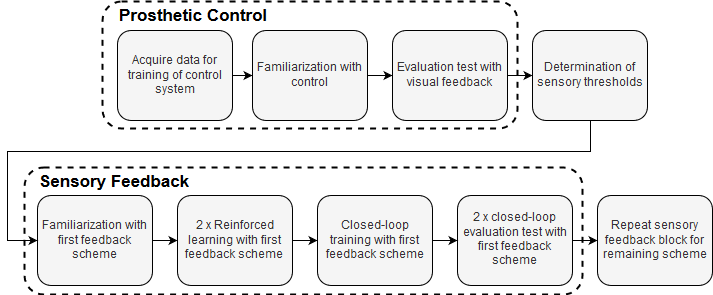
\includegraphics[width=.47\textwidth]{figures/std_paper}
	\caption{Pipeline showing the stages of the experiment. The stages in the first block focused on developing and evaluating a subject specific simulated prosthetic control system. Then electrotactile sensory thresholds were determined. The second block focused on training the understanding of the feedback schemes and evaluating their use in combination with prosthetic control.}
	\label{fig:std_pap} 
\end{figure}

During the first block, EMG data was initially acquired and used to train a control system, which was used for a simulate prosthetic control. Subsequently, was a stage where the subject was made familiar with the control system. Finally, the achieved prosthetic control was evaluated through a target reaching test. Afterwards, a series of subjects sensory thresholds were determined for use of conveying electrotactile feedback. The subject then began the stages of familiarizing and training with a feedback scheme followed by re-familiarization of control in combination with feedback. Finally, a evaluation test of using the sensory feedback in combination for control was made. The entire sensory feedback block was then repeated using the remaining feedback scheme. 



	
	\subsection{Novel Feedback Configurations}
The main objective of the study was to evaluate the effectiveness of two novel electrotactile feedback configurations in providing proprioceptive information of a two DoF myoelectric prosthesis. 
The DoF's used were wrist rotation and hand aperture. The transmitted feedback was discrete, where the full range of each feedback variable was been divided into five segments. The electrode array used to deliver electrical stimulation can be seen in figure \ref{fig:pa:electrode}.
\begin{figure}[H]                 
	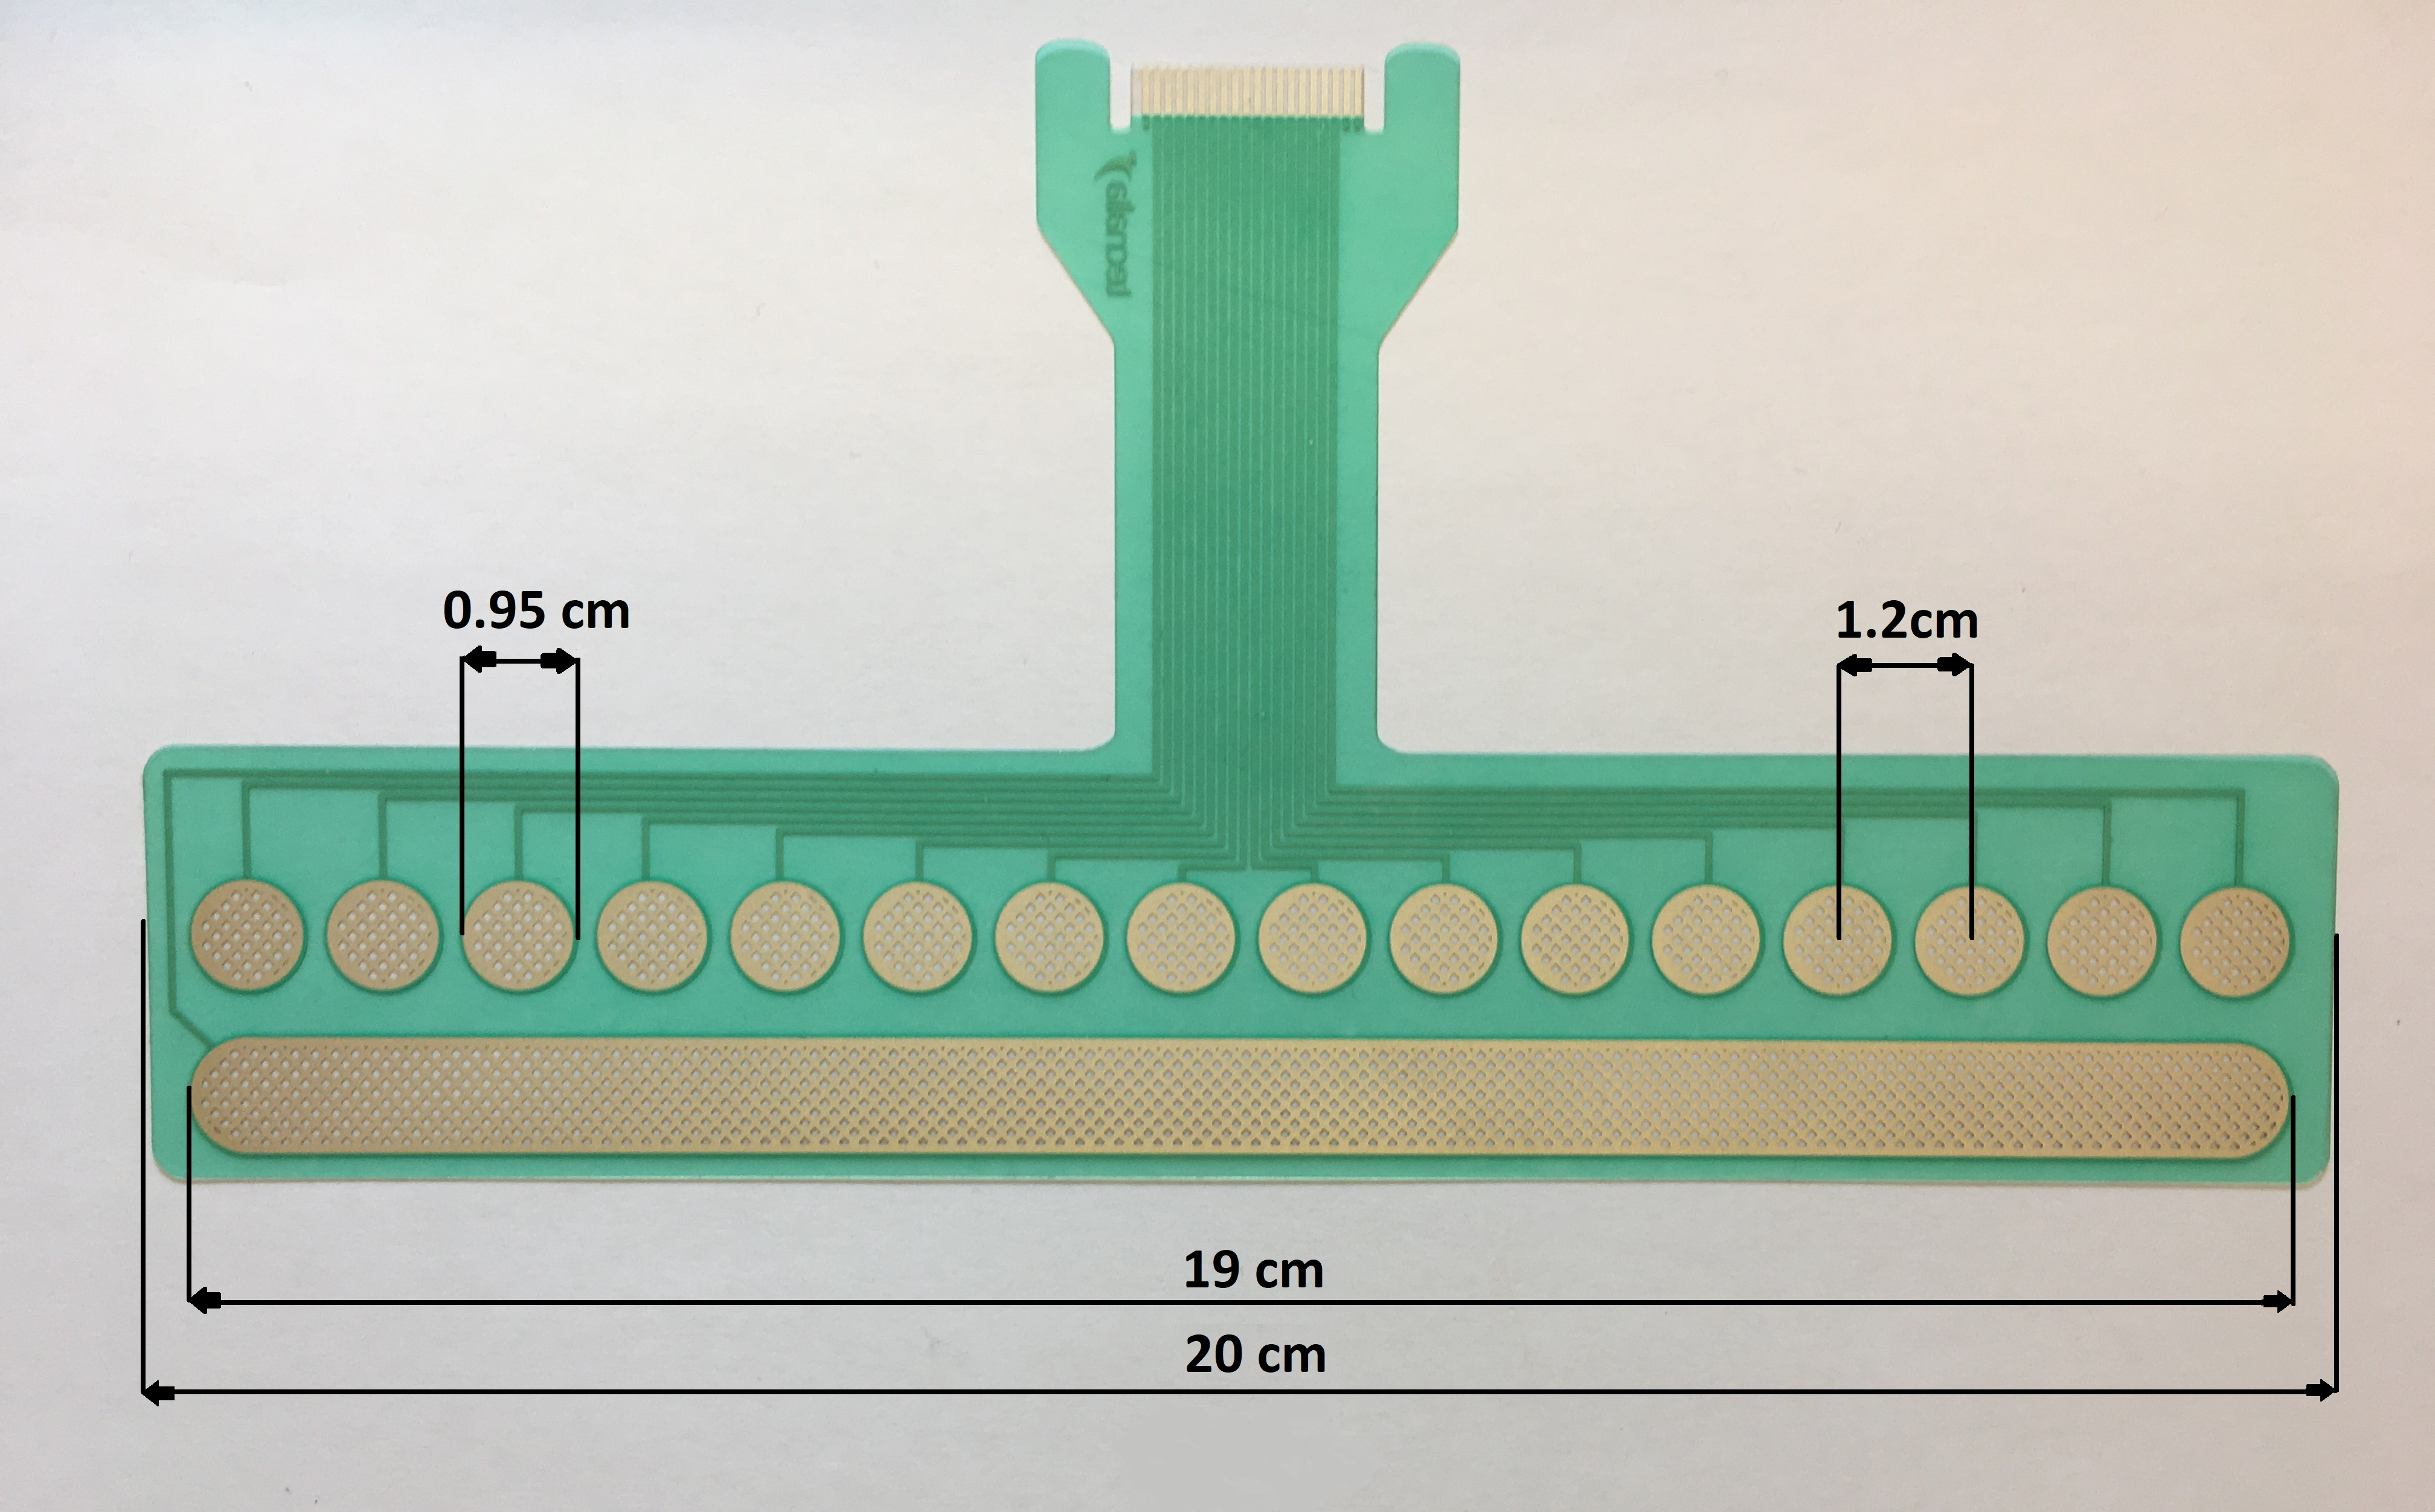
\includegraphics[width=1\textwidth]{figures/electrode}  
	\caption{Image of the 16 multi-pad electrode array used for stimulation. It consisted of 16 circular cathode pads, which each shared a common anode.}
	\label{fig:pa:electrode} 
\end{figure}
\begin{figure}[h]                 
	\includegraphics[width=1\textwidth]{figures/max}  
	\caption{The MaxSense stimulation device used for independently controlling the activation of each pad in the attached electrode array.}
	\label{fig:pa:max} 
\end{figure}   
The array electrode consisted of a single anode pad and 16 circular cathode pads. The pads comprised of conductive Ag/AgCl traces imprinted in a 150 $\mu$m thick polyester layer. All pads were covered with conductive hydrogel (AG702, Axelgaard, Denmark) to enhance skin-electrode contact.  A multichannel stimulation feedback device (MaxSens, Tecnalia, Spain), seen in figure \ref{fig:pa:max}, generating biphasic pulses was connected to a standard desktop PC for individual control of pad activation. The pulse width and amplitude could be modulated independently for each pad whereas the frequency was controlled globally. The pulse width could be modulated within a 50 - 1000 $\mu $s range with 10 $\mu $s steps, frequency ranges from 1 - 400 Hz with 1 Hz steps and current amplitude ranges from 50 - 10000 $\mu $A with 0.1 $\mu $A steps. The array electrode was placed circumferentially around the non-dominant arm to avoid interference with the EMG electrodes, which were fitted on the dominant arm. In a clinical application both interfaces should be placed on the same arm (residual limb). The stimulation electrodes were fitted such that the end pads had a maximum gap of 3 cm centrally on the volar side, when using a pronated arm as reference position. Hence, how distal the electrode array was placed towards the wrist depended on the diameter of the subject's forearm. The following sections will present the two developed feedback configurations. 


\subsubsection{Spatial configuration}

The motivation behind the spatial configuration was to communicate wrist rotation by spatially rotating dorsally placed active electrode pads and to communicate hand aperture by changing activation between volarly placed pads. 
This feedback design was chosen in order to intuitively mimic the directions of the motions in the included DoF's. An illustration of the spatial configuration can be seen in figure \ref{fig:pa:spatial}. The pads were divided into two groups each responsible for conveying information about a single DoF. The dorsally placed pads were allocated for wrist rotation and the volarly placed for hand aperture. The pads were furthermore paired such that each pair would represent one of four intervals of the feedback variable. For wrist rotation the pads were connected in side by side pairs. For right-handed subjects the activation of pad pairs would rotate laterally when increasing rotational states during supination and rotate medially during pronation. For the hand aperture DoF the pairs consisted of oppositely located pads on the medial and lateral sides. When increasing aperture states the active pairs would move volarly and the distance between active pads would become shorter. When both feedback variables were active, the pads pairs corresponding to the level of the hand aperture and rotational angle would be activated. Thus, a maximum of four pads could be active simultaneously. The reason for grouping adjacently placed pads to convey information about the rotational DoF was to improve sensation perception by stimulating a larger skin area, as shown in Dosen et al. \cite{Dosen2015}. 
\begin{figure}[h]                 
	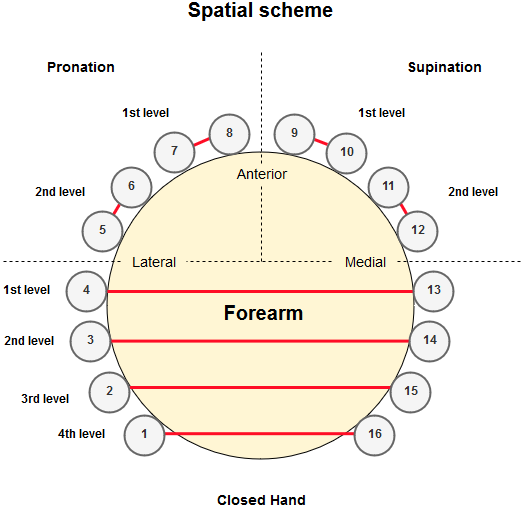
\includegraphics[width=.9\textwidth]{figures/El_array_spatial}  
	\caption{Transverse view of the developed spatial scheme fitted on the left arm of a subject. The levels written next to the pads pairs corresponded to the level of the position state; the higher the level, the higher the position state of the given movement was. When fitted on the right arm medial and lateral sides were reversed.}
	\label{fig:pa:spatial} 
\end{figure}   

\subsubsection{Amplitude configuration}
The incentive behind the amplitude configuration was to convey information by increasing the amplitude as the feedback variable increased. The feedback was provided in electrode pad groups of four.
The areas of active pads allocated for the various motions was similar to the spatial configuration to intuitively resemble the prosthesis motions. An illustration of the amplitude configuration can be seen in figure \ref{fig:pa:amplitude}. 
 \begin{figure}[h]                 
	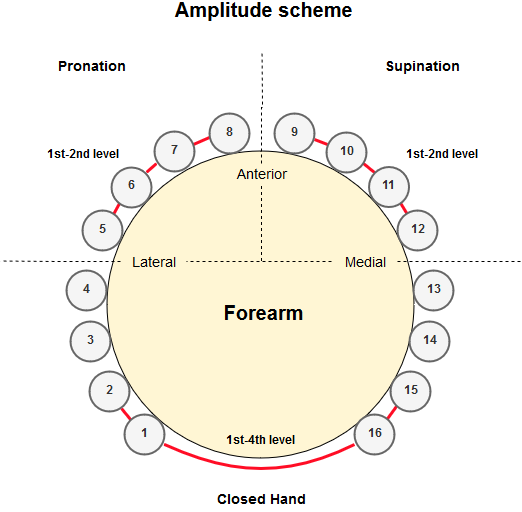
\includegraphics[width=.9\textwidth]{figures/El_array_amplitude}  
	\caption{Transverse view of the developed amplitude scheme fitted on the left arm of a subject. Different groups of four electrode pads were active during supination, pronation and hand aperture, respectively. The amplitude of the active pads would increase with the increase of the position state; the higher the position state level the higher the current amplitude of the given pads. When fitted on the right arm medial and lateral sides were reversed.}
	\label{fig:pa:amplitude} 
\end{figure}

The eight most dorsally placed pads were used for wrist rotation and the four most volarly placed pads for hand aperture. The eight pads used during wrist rotation were split such that the four most laterally placed were used during supination and four most medially placed were used during pronation for right-handed subjects. The pad activation was reversed for left-handed subjects. As the position state of a given movement would increase the current amplitude in the pads corresponding to that movement would increase. When in combined DoF position states, the pads corresponding to the level of the position state of each DoF would be active in the relative amplitude level. Thus, a maximum of eight pads could be active concurrently. The choice of grouping four electrode pads was decided upon to exploit the highest number of pads in the electrode array, while maintaining a symmetric distribution of possible active pads. Similarly to the spatial configuration this design was chosen to improve sensation perception \cite{Dosen2015}.



	
	
\subsection{Virtual Closed-Loop Prosthesis}
 \begin{figure*}[h]
		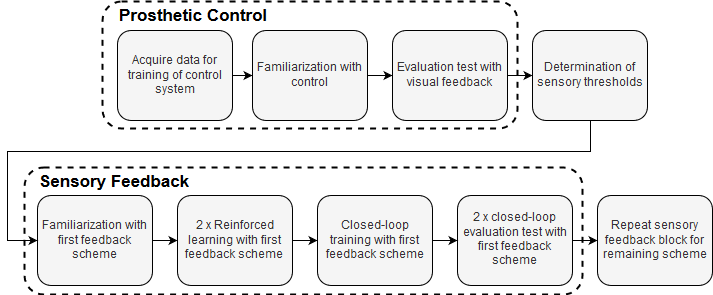
\includegraphics[width=.85\textwidth]{figures/std_paper}
	\caption{Pipeline showing the stages of the experiment. The stages in the first block focused on developing a prosthetic control system, and evaluating the subjects' ability to control the prosthesis. Then electrotactile sensory thresholds were determined. The second block focused on training the understanding of the feedback schemes and evaluating their use in combination with prosthetic control. The sensory feedback block was repeated for the remaining feedback scheme.}
	\label{fig:pa:std_pap} 
\end{figure*}
Investigating the usability of the two sensory configurations in a closed-loop scenario required these to be interfaced with a prosthetic device, which accommodated the actuation of rotational and hand aperture DoF's. However, using an actual prosthesis might result in auditory feedback being provided to the subject through prosthetic actuation sounds, eliminating the interest of solely exploring the impact of tactile feedback. Hence, it was chosen to simulate a velocity-based virtual prosthesis which enabled evaluation of the developed feedback schemes. In figure \ref{fig:pa:gridmap} is a depiction of a grid system, where the axes corresponded to the rotation angles and hand aperture. The grid squares represented the discrete intervals that were communicated through the feedback, where the cursor was the current angle and hand aperture. 
\begin{figure}[H]                 
	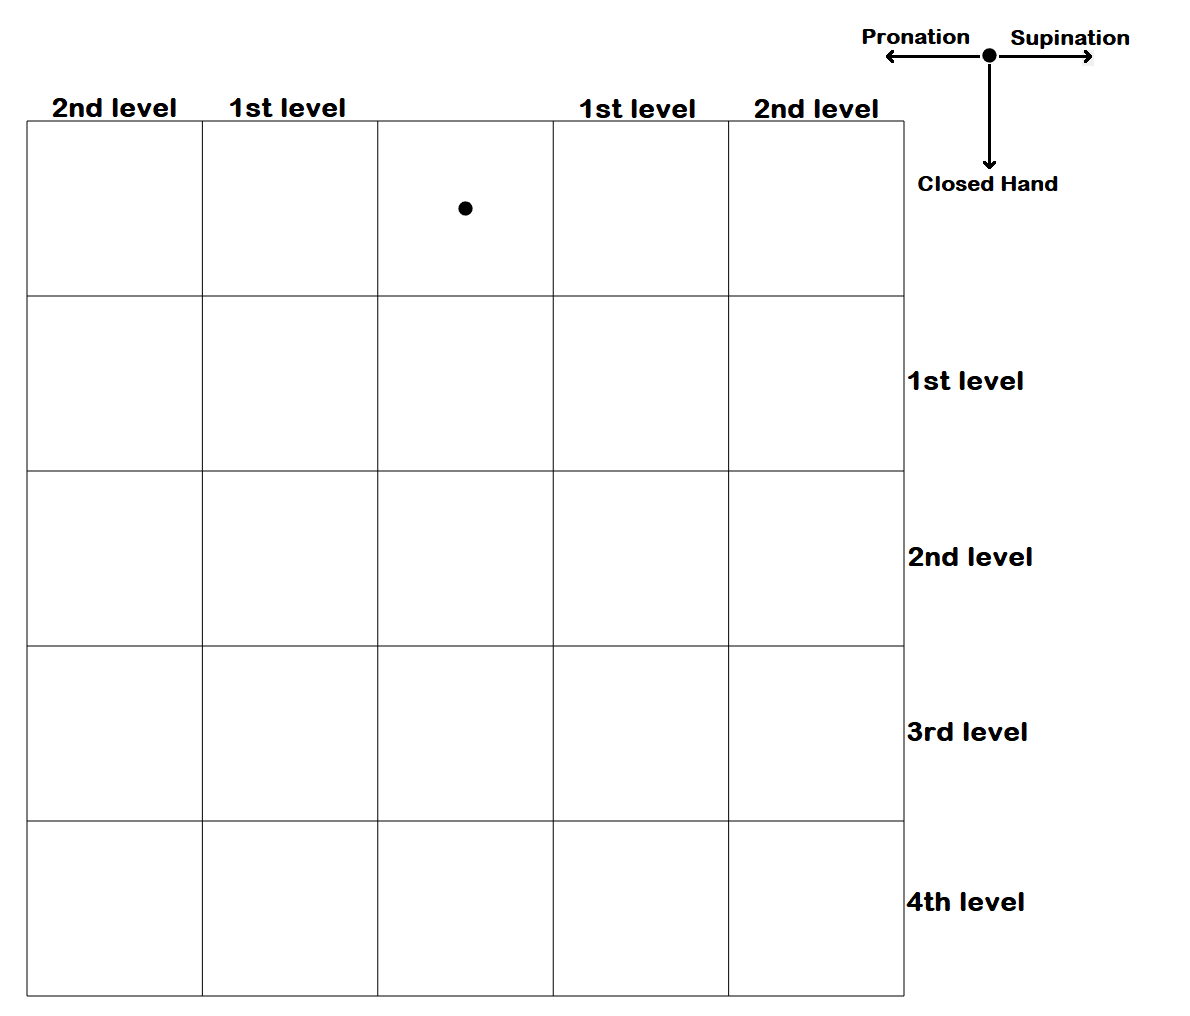
\includegraphics[width=1\textwidth]{figures/gridmap2}  
	\caption{Image of the grid map and cursor used in the experiment. Wrist supination moved the cursor to the right, pronation moved it to the left and closing the hand moved it downwards. For left-handed subjects, the rotational movements were reversed. Opening the hand moved the cursor upwards, and was used as a correction movement if needed.}
	\label{fig:pa:gridmap} 
\end{figure}

Performing supination would make the cursor move to the right and to the left when performing pronation. Performing closed hand would make the cursor move downwards and upwards when performing open hand, resembling the change in hand aperture. Performing rest (relaxing the arm) would make the cursor stand still. Furthermore, the contraction intensity was made proportional with the actuation speed, enabling the subject to have greater control of cursor movement speed. The control was sequential which only enabled the cursor to move in one DoF at a time. The control scheme thereby resembles what is typically used in commercial prostheses \cite{Atzori2015}. When the cursor entered a square a specific electrotactile stimulation would be provided corresponding to the stimulation pattern for each scheme. In the neutral position (location of cursor in figure \ref{fig:pa:gridmap}), no tactile feedback was provided.     


	
	
	
	\section*{IV. RESULTS}%%%%%%%%%%%%%%%%%%%%%%%%%%%%%%%%%%%%%%%%%%%%%%%%%%%%%%%%%%%%%%%%%%%
	%\input{contents/zxPaper/ResultsPaper.tex}
	
	
	%\begin{multicols}{2}
	\section*{V. DISCUSSION}%%%%%%%%%%%%%%%%%%%%%%%%%%%%%%%%%%%%%%%%%%%%%%%%%%%%%%%%%%%%%%%%
	
	%\input{contents/cResults/discussion.tex}
	
	\subsection*{VI. CONCLUSION}%%%%%%%%%%%%%%%%%%%%%%%%%%%%%%%%%%%%%%%%%%%%%%%%%%%%%%%%%%%%%%%
	
%	\input{contents/cResults/conclusion.tex}
	
	%%%%%%%%%%%%%%%%%%%%%%%%%%%%%%%%%%%%%%%%%%%%%%%%%%%%%%%%%%%%%%%%%%%%%%%%%%%%%%%%
	
	
	\subsection*{ACKNOWLEDGMENT}
	
	The authors would like to thank supervisors Strahinja Dosen and Jakob Lund Dideriksen for providing constructive feedback, and the School of Medicine and Health at Aalborg University for providing equipment and the facilities to complete this study. Additionally, the authors are very thankful for all the voluntary participants. 


\renewcommand*{\bibfont}{\small}
	\urlstyle{same}
	\printbibliography
	

	%			\bibitem{citeKey} author, title, publisher , volume, year
	
	%	\begin{thebibliography}{99}				
	%		\bibitem{Fougner2012} Fougner, Anders and Stavdahl, Oyvind and Kyberd, Peter J. and Losier, Yves G. and Parker, Philip A., Control of upper limb prostheses: Terminology and proportional myoelectric control a review, IEEE Trans. Neural Syst. Rehabil. Eng., 20, 2012
	%		\bibitem{amsuess2014} Amsuess, Sebastian and Goebel, Peter and Graimann, Bernhard and Farina, Dario, Extending mode switching to multiple degrees of freedom in hand prosthesis control is not efficient, 2014
	%		\bibitem{Ison2016} Ison, M and Vujaklija, I and Whitsell, B and Farina, D, High-density electromyography and motor skill learning for robust long-term control of a 7-DoF robot arm, IEEE Trans., 24, 2016
	
	%	\end{thebibliography}
	%	
\end{multicols}

\end{document}
